% Week 62 materials: activity cards A-H and slot headers 1-4, three kits per sheet.
% Print on card stock and cut on the lines. Each cell is 31 mm by 38 mm.
\documentclass[12pt,letterpaper]{article}
\usepackage[margin=0.5in,top=0.72in,bottom=0.65in,headheight=17pt,headsep=10pt]{geometry}
\usepackage[T1]{fontenc}
\usepackage{helvet}
\renewcommand{\familydefault}{\sfdefault}
\usepackage{tikz}
\usepackage{fancyhdr}
\pagestyle{fancy}
\fancyhf{}
\fancyhead[L]{\small Week 62 / Conflict networks / Materials}
\fancyfoot[L]{\footnotesize Bellingham Math Circle / Week 62 / W62-M-v1}
\fancyfoot[R]{\footnotesize\thepage}
\renewcommand{\headrulewidth}{0.4pt}
\renewcommand{\footrulewidth}{0pt}
\setlength{\parindent}{0pt}
% \cell{column}{row}{content}: one 31 x 38 mm cut cell, row 0 at the top.
\newcommand{\cell}[3]{\begin{scope}[shift={({(#1)*31},{-(#2)*38})}]#3\end{scope}}
% An activity card: one large letter.
\newcommand{\activity}[1]{\node[font=\fontsize{56}{56}\selectfont] at (15.5,-19) {#1};}
% A slot header: its number, and a circle where one counter of the slot's colour sits.
\newcommand{\header}[1]{%
  \node[font=\small] at (15.5,-5) {slot};
  \node[font=\fontsize{34}{34}\selectfont\bfseries] at (15.5,-14.5) {#1};
  \draw[dashed,line width=0.5pt] (15.5,-28.5) circle (8);}
\begin{document}
\begin{center}
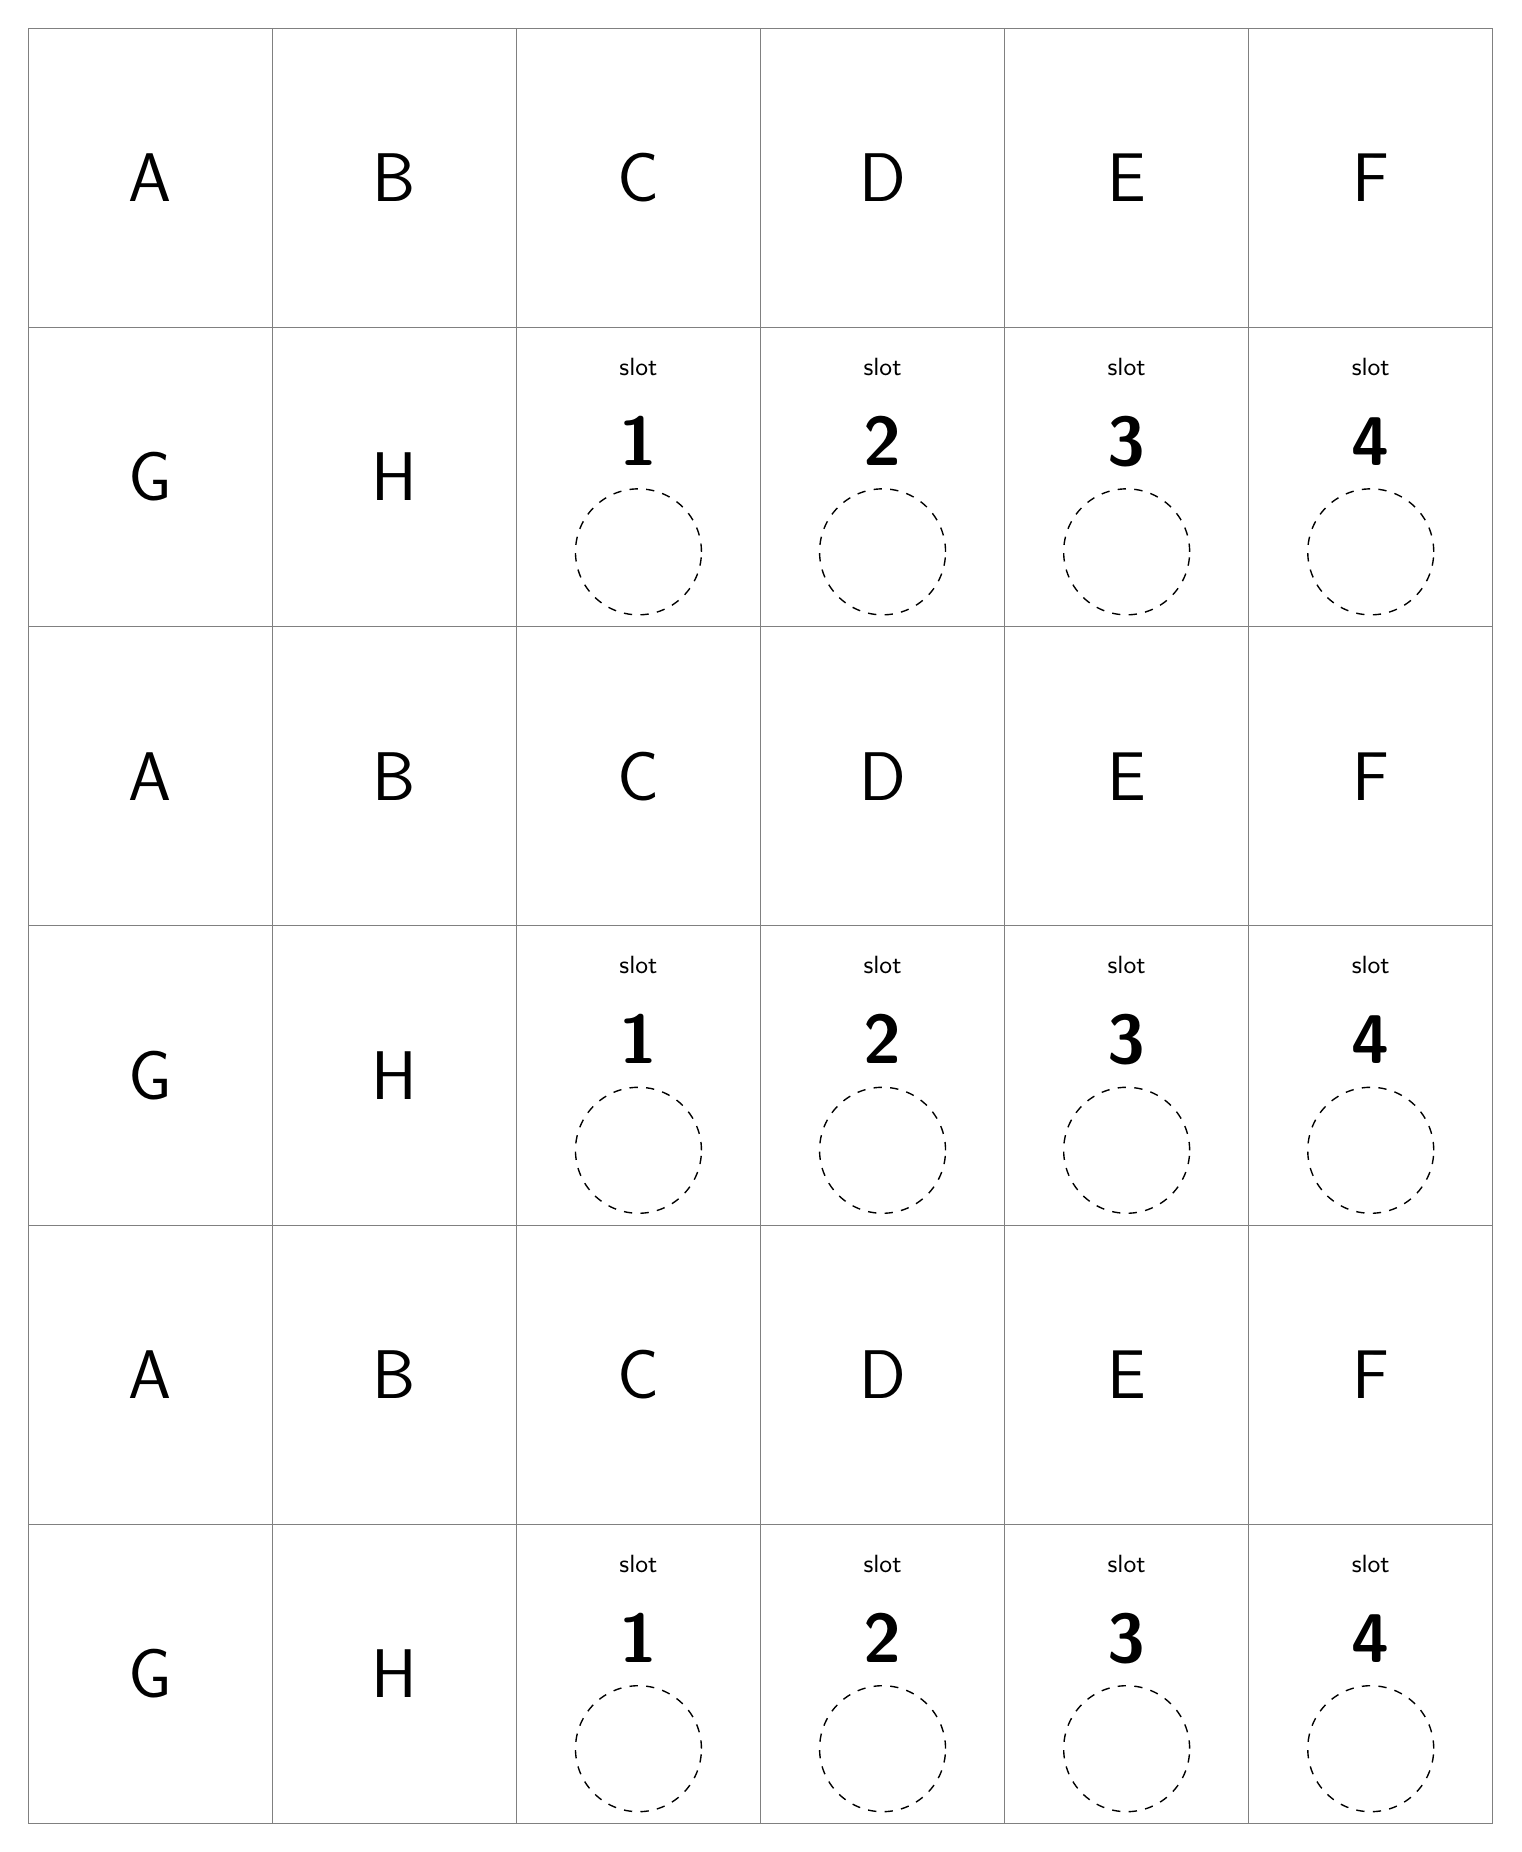
\begin{tikzpicture}[x=1mm,y=1mm]
\foreach \kit in {0,1,2}{
  \foreach \letter [count=\i from 0] in {A,B,C,D,E,F}{\cell{\i}{2*\kit}{\activity{\letter}}}
  \cell{0}{2*\kit+1}{\activity{G}}
  \cell{1}{2*\kit+1}{\activity{H}}
  \foreach \n [count=\i from 2] in {1,2,3,4}{\cell{\i}{2*\kit+1}{\header{\n}}}
}
\draw[gray,line width=0.4pt,step=1] (0,0) grid[xstep=31,ystep=38] (186,-228);
\end{tikzpicture}
\end{center}
\end{document}
